\newpage
\maketitle
\begin{center}
\Large \textbf{第3章 GARCH模型} \quad 
\end{center}
\begin{abstract}
在本章中我们将首先讲述条件异方差模型GARCH(Generalized AutoRegressive Conditional Heteroskedastic),
并将GARCH模型用于实际金融时间序列数据拟合。
\end{abstract}
\section{GARCH模型}
我们之前讨论的时序信号,都是假定其为平稳的。但是有很多时序信号,如某些商品的需求或价格,会随着季节的变化而发生变化,股票的价格为出现长时间的上涨或下跌趋势,在这些情况下,使用ARIMA模型的效果就不太好。对于我们要研究的股票数据,由于市场上很多交易是由大机构的算法来进行交易的,当出现价格明显示上涨或下跌时,会自动触发这些算法进行交易,从而放大了这种上涨或下跌趋势。这种情况我们称之为异方差,研究这种现象的方法我们称之为通用自回归条件异方差GARCH(Generalized AutoRegression Conditional Heteroskedasticity)模型。
\subsection{定义}
\subsubsection{ARCH模型}
我们先来看较为简单的自回归条件异方差ARCH模型,我们假设时序信号如下所示:
\begin{equation}
\epsilon _{t} = \sigma _{t} w_{t}
\label{e000050}
\end{equation}
其中$w_{t}$为白噪声序列,$\sigma _{t}$的定义如下所示:
\begin{equation}
\sigma _{t}^{2} = \alpha _{0} + \alpha _{1} \epsilon _{t-1}^{2}
\label{e000051}
\end{equation}
这个模型我们称之为ARCH(1)模型。我们以这个简单的模型为例,来说明ARCH(1)模型是对时序信号方差的变化进行建模。
我们首先来看时间序列$\{ \epsilon _{t} \}$的均值:
\begin{equation}
E(\epsilon _{t}) = E(\sigma _t w_{t}) = E(\sigma _{t})E(w_{t})=0
\label{e000052}
\end{equation}
我们再来看时间序列$\{ \epsilon _{t} \}$的方差:
\begin{equation}
\begin{aligned}
Var(\epsilon _{t}) = E\big( \epsilon _{t} - E(\epsilon _{t}) \big)^{2} =E\big( \epsilon _{t}^{2} - 2\epsilon _{t}E(\epsilon _{t}) + (E(\epsilon _{t}))^{2} \big) \\
=E(\epsilon _{t}^{2})-2E(\epsilon _{t})E(\epsilon _{t})+(E(\epsilon _{t}))^{2}=E(\epsilon _{t}^{2})-(E(\epsilon _{t}))^{2} \\
=E(\epsilon _{t}^{2})=E(\sigma _{t}^{2}w_{t}^{2})=E(\sigma _{t}^{2})E(w_{t}^{2})=E(\alpha _{0} + \alpha _{1}\epsilon _{t-1}^{2}) \\
=\aleph _{0} + \alpha _{1}E(\epsilon _{t-1}^{2})=\alpha _{0} + \alpha _{1}Var(\epsilon _{t-1})
\end{aligned}
\label{e000053}
\end{equation}
在上面的公式推导中,我们用到了$\{ w_{t} \}$为白噪声信号,其均值为0,方差为1。\newline
了解了基本ARCH模型之后,我们可以将ARCH(1)模型扩展到ARCH(p)模型,这里我们就不再展开了,将在下一节GARCH模型中进行详细介绍。
\subsubsection{GARCH模型}
对于时间序列信号$\{ \epsilon _{t} \}$其表达式为:
\begin{equation}
\epsilon _{t} = \sigma _{t} w_{t}
\label{e000054}
\end{equation}
其中$\{ w_{t} \}$为白噪声信号,其均值为0方差为1。其$\sigma _{t}^{2}$的定义为:
\begin{equation}
\sigma _{t}^{2} = \alpha _{0} + \sum_{i=1}^{p} \alpha _{i} \epsilon _{t-i}^{2} + \sum_{j=1}^{q} \beta _{j} \sigma _{t-j}^{2}
\label{e000055}
\end{equation}
其中$\alpha _{0}$、$\alpha _{i}$、$\beta _{j}$为参数。
\subsection{数据模拟}
为了对问题进行简化,我们在这里只模拟GARCH(1,1)模型,具体欲模拟的时间序列信号如下所示,在arch包的GARCH模型中,我们研究的信号为$r_{t}$,并且多出一个参数$\mu$:
\begin{equation}
\begin{aligned}
r_{t} = \epsilon _{t} + \mu \\
\epsilon _{t} = \sigma _{t}w_{t} \\
\sigma _{t}^{2} = \omega + \alpha _{1} \epsilon _{t-1}^{2} + \beta _{1} \sigma _{t-1}^{2}=0.2 + 0.5\epsilon _{t-1}^{2} + 0.3\sigma _{t-1}^{2}
\end{aligned}
\label{e000056}
\end{equation}
其程序如下所示:
\lstset{language=PYTHON, caption={GARCH拟合模拟数据}, label={c000008}}
\begin{lstlisting}
import sys
import math
import numpy as np
import pandas as pd
from pandas.plotting import register_matplotlib_converters
import matplotlib.pyplot as plt
import matplotlib.dates as mdates
from matplotlib.font_manager import FontProperties
from statsmodels.tsa import stattools
from statsmodels.graphics import tsaplots
from statsmodels.tsa.arima_model import ARIMA
import arch.unitroot as unitroot
import arch as arch

class Aqt002(object):
    def __init__(self):
        self.name = 'Aqt001'
        # 数据文件格式:编号 日期 星期几 开盘价 最高价 
        # 最低价 收益价 收益
        # Indexcd	Trddt	Daywk	Opnindex	Hiindex	
        # Loindex	Clsindex	Retindex
        self.data_file = 'data/pqb/aqt002_001.txt'
        
    def startup(self):
        print('GARCH模型...')
        np.random.seed(1)
        alpha0 = 0.2
        alpha1 = 0.5
        beta1 = 0.3
        samples = 10000 # 样本数量
        w = np.random.standard_normal(size=samples)
        epsilon = np.zeros((samples,), dtype=float)
        sigma = np.zeros((samples,), dtype=float)
        for i in range(2, samples):
            sigma_2 = alpha0 + alpha1 * math.pow(epsilon[i-1], 2) + \
                        beta1 * math.pow(sigma[i-1], 2)
            sigma[i] = math.sqrt(sigma_2)
            epsilon[i] = sigma[i]*w[i]
        plt.title('epsilon signal')
        plt.plot(epsilon)
        plt.show()
        # 绘制epsilonACFS
        acfs = stattools.acf(epsilon)
        tsaplots.plot_acf(epsilon, use_vlines=True, lags=30)
        plt.title('epsilon ACF')
        plt.show()
        # 绘制epsilon pow2 ACF
        acfs2 = stattools.acf(np.power(epsilon, 2))
        tsaplots.plot_acf(np.power(epsilon, 2), use_vlines=True, lags=30)
        plt.title('pow(epsilon,2) ACF')
        plt.show()
        # GARCH拟合
        am = arch.arch_model(epsilon, x=None, mean='Constant', 
                    lags=0, vol='Garch', p=1, o=0, q=1, 
                    power=2.0, dist='Normal', hold_back=None)
        model = am.fit(update_freq=0)
        # GARCH(1,1)参数
        print('############ GARCH(1,1)参数  ###################')
        print('model_type:{0}'.format(type(model)))
        print('mu={0:0.2f}; a0={1:0.2f}; a1={2:0.2f}; b1={3:0.2f}' \
                    .format(model.params['mu'], model.params['omega'], 
                    model.params['alpha[1]'], model.params['beta[1]']   ))
        print('###############################')
        #print(model.summary())
        # 残差信号
        plt.title('GARCH(1,1) resid')
        plt.plot(model.resid)
        plt.show()
        # 残差ACF
        resid_acf = stattools.acf(model.resid)
        tsaplots.plot_acf(model.resid, use_vlines=True, lags=30)
        plt.title('GARCH(1,1) resid ACF')
        plt.show()
        # ADF检验
        resid_adf = unitroot.ADF(model.resid)
        print('stat={0:0.4f} vs 1%_cv={1:0.4f}'.format( \
                    resid_adf.stat, resid_adf.critical_values['1%']))
        if resid_adf.stat < resid_adf.critical_values['1%']:
            print('resid为稳定时间序列 ^_^')
        else:
            print('resid为非稳定时间序列!!!!!')
        # Ljung-Box检验
        resid_ljung_box = stattools.q_stat(stattools.acf( \
                    model.resid)[1:12], len(model.resid))
        resid_lbv = resid_ljung_box[1][-1]
        print('resid_ljung_box_value={0}'.format(resid_lbv))
        # 0.05为显著性水平
        if resid_lbv < 0.05:
            print('resid为平稳时间序列 ^_^')
        else:
            print('resid为非平稳时间序列!!!!!!!')
        # 预测
        y = model.forecast(horizon=3)
        print('########### 预测值  ###############')
        print('len={0}; p1={1:0.3f}; p2={2:0.3f}; p3={3:0.3f}'. \
                    format(len(y.mean.iloc[-1]), y.mean.iloc[-1][0], 
                    y.mean.iloc[-1][1], y.mean.iloc[-1][2]))
        print('##########################')
\end{lstlisting}
我们欲拟合的时间序列信号为:
\begin{figure}[H]
	\caption{拟拟合的时间序列}
	\label{f000031}
	\centering
	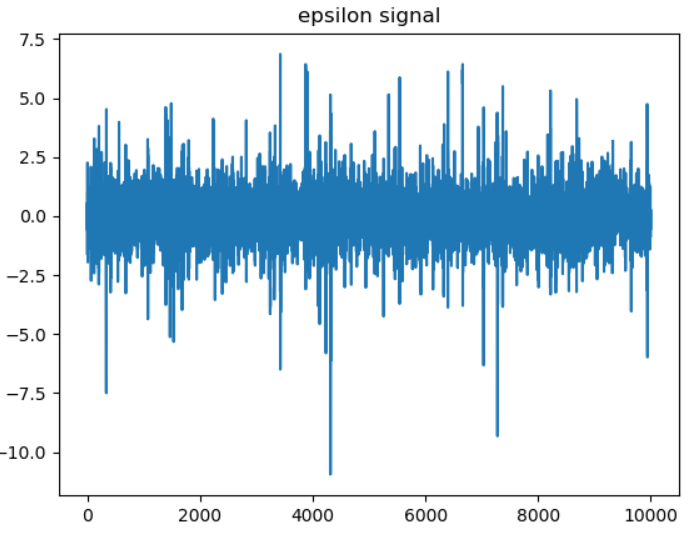
\includegraphics[height=2cm]{images/f000031}
\end{figure}
该时间序列的自相关系数函数ACF图:
\begin{figure}[H]
	\caption{epsilon的自相关系数函数ACF图}
	\label{f000032}
	\centering
	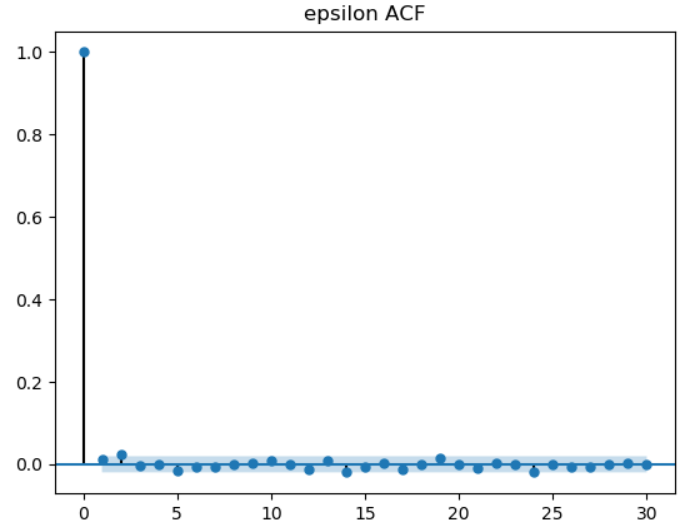
\includegraphics[height=2cm]{images/f000032}
\end{figure}
由上图可以看出,其基本是一个平稳时间序列。我们取其平方,其自相关系数函数ACF图如下所示:
\begin{figure}[H]
	\caption{pow(epsilon,2)的自相关系数函数ACF图}
	\label{f000033}
	\centering
	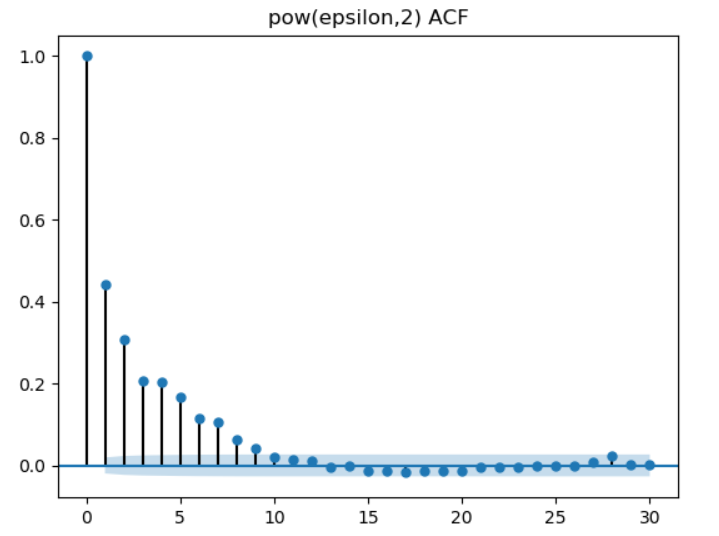
\includegraphics[height=2cm]{images/f000033}
\end{figure}
由上图可以看出,将其平方后,其就是不平稳的时间序列了。GARCH模型就是来处理这种情况的。\newline
我们采用GARCH进行拟合后,得到的残差信号为:
\begin{figure}[H]
	\caption{GARCH(1,1)残差序列}
	\label{f000034}
	\centering
	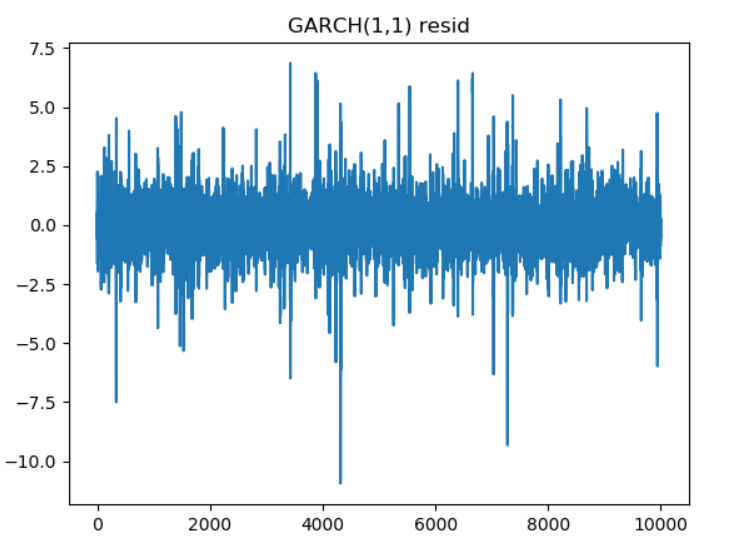
\includegraphics[height=2cm]{images/f000034}
\end{figure}
残差信号的自相关系数函数ACF图为:
\begin{figure}[H]
	\caption{GARCH(1,1)残差序列自相关系数函数ACF图}
	\label{f000035}
	\centering
	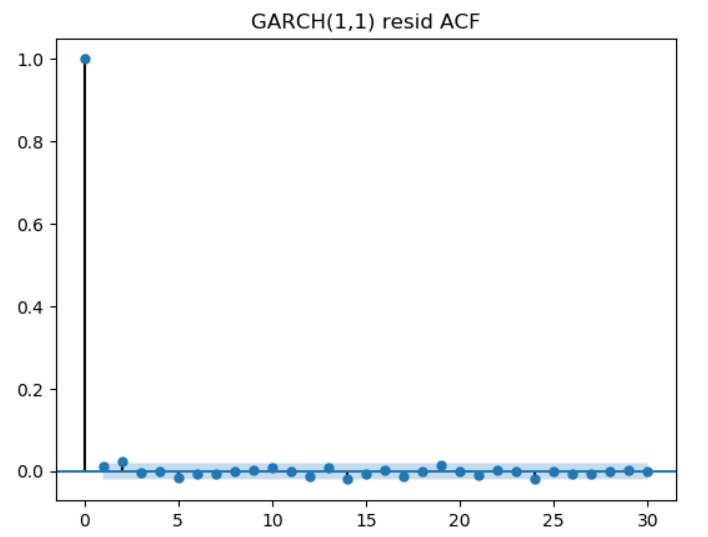
\includegraphics[height=2cm]{images/f000035}
\end{figure}
程序的运行结果如下所示:
\begin{figure}[H]
	\caption{程序运行结果}
	\label{f000036}
	\centering
	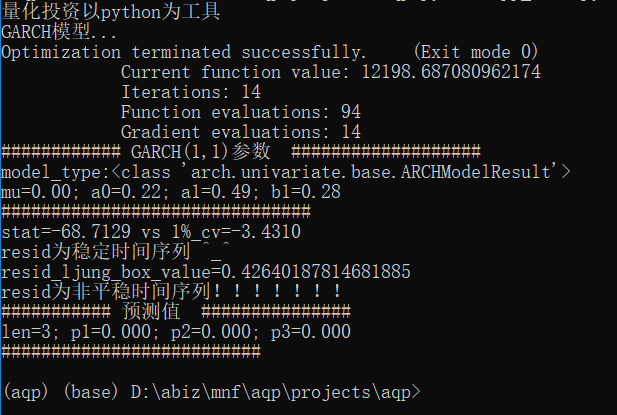
\includegraphics[height=2cm]{images/f000036}
\end{figure}
由上图可知,我们对GARCH(1,1)模型的参数预测还是相当准确的,说明我们方法是正确的。
\subsection{金融数据拟合}
下面我们以上证综指的收盘价为例,来讨论GARCH拟合预测后三天股价问题。对于收盘价这样的信号,我们仍然采用对数一阶差分形式来作为建模的时间序列,我们用GARCH(3,2)来进行拟合,程序如下所示:
\lstset{language=PYTHON, caption={GARCH拟合并预测上证综指收盘价}, label={c000009}}
\begin{lstlisting}
    def garch_finance_demo(self):
        print('拟合上证综指收盘价...')
        register_matplotlib_converters()
        data = pd.read_csv(self.data_file, sep='\t', index_col='Trddt')
        sh_index = data[data.Indexcd==1]
        sh_index.index = pd.to_datetime(sh_index.index)
        sh_return = sh_index.Retindex
        # raw_data = sh_index.Retindex
        raw_data = sh_index.Clsindex
        train_data = raw_data[:-3]
        dcp = np.log(train_data).diff(1)[1:] 
        plt.plot(dcp)
        plt.show()
        # GARCH拟合
        am = arch.arch_model(dcp, x=None, mean='Constant', 
                    lags=0, vol='Garch', p=3, o=0, q=2, 
                    power=2.0, dist='Normal', hold_back=None)
        model = am.fit(update_freq=0)
        # GARCH(1,1)参数
        print('############ GARCH(1,1)参数  ###################')
        '''
        print('mu={0:0.2f}; a0={1:0.2f}; a1={2:0.2f}; a2={3:0.2f}, b1={4:0.2f}, b2={5:0.2f}' \
                    .format(model.params['mu'], model.params['omega'], 
                    model.params['alpha[1]'], model.params['alpha[2]'], model.params['beta[1]'], model.params['beta[2]']   ))
        '''
        print('###############################')
        resid = model.resid
        # 绘制ACF
        acfs = stattools.acf(resid)
        print(acfs)
        tsaplots.plot_acf(resid, use_vlines=True, lags=30)
        plt.title('GARCH(p,q) ACF figure')
        plt.show()
        '''
        pacfs = stattools.pacf(resid)
        print(pacfs)
        tsaplots.plot_pacf(resid, use_vlines=True, lags=30)
        plt.title('ARIMA(p,d,q) PACF figure')
        plt.show()
        '''
        # ADF检验
        resid_adf = unitroot.ADF(resid)
        print('stat={0:0.4f} vs 1%_cv={1:0.4f}'.format(resid_adf.stat, resid_adf.critical_values['1%']))
        if resid_adf.stat < resid_adf.critical_values['1%']:
            print('resid为稳定时间序列 ^_^')
        else:
            print('resid为非稳定时间序列!!!!!')
        # Ljung-Box检验
        resid_ljung_box = stattools.q_stat(stattools.acf(resid)[1:12], len(resid))
        resid_lbv = resid_ljung_box[1][-1]
        print('resid_ljung_box_value={0}'.format(resid_lbv))
        # 0.05为显著性水平
        if resid_lbv < 0.05:
            print('resid为平稳时间序列 ^_^')
        else:
            print('resid为非平稳时间序列!!!!!!!')
        # 预测
        frst = model.forecast(horizon=3)
        y = frst.mean.iloc[-1]
        print('预测值:{0}'.format(y))
        p1 = math.exp(math.log(train_data[-1]) + y[0])
        p2 = math.exp(math.log(p1) + y[1])
        p3 = math.exp(math.log(p2) + y[2])
        print('        预测值    实际值  (3957.534)')
        print('第一天:{0} vs 4034.310'.format(p1))
        print('第二天:{0} vs 4121.715'.format(p2))
        print('第三天:{0} vs 4135.565'.format(p3))
\end{lstlisting}
我们要建模的上证综指收盘价对数差分信号如下所示:
\begin{figure}[H]
	\caption{上证综指收盘价对数差分信号}
	\label{f000037}
	\centering
	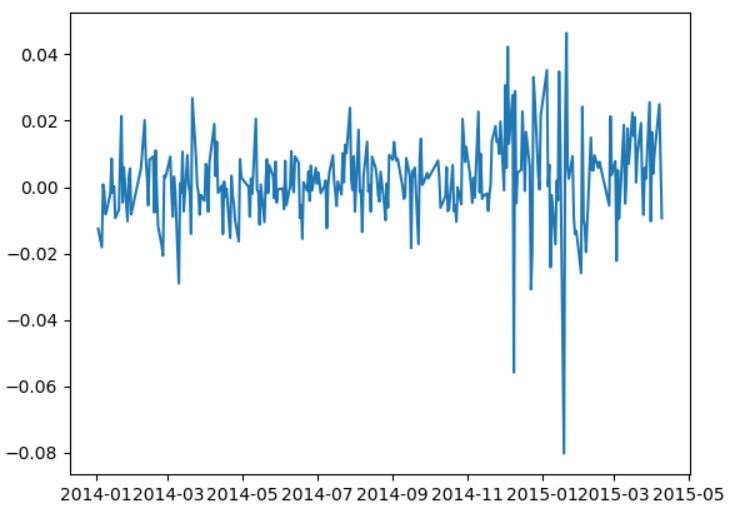
\includegraphics[height=2cm]{images/f000037}
\end{figure}
经过GARCH(3,2)拟合后的残差信号:
\begin{figure}[H]
	\caption{上证综指收盘价对数差分信号}
	\label{f000038}
	\centering
	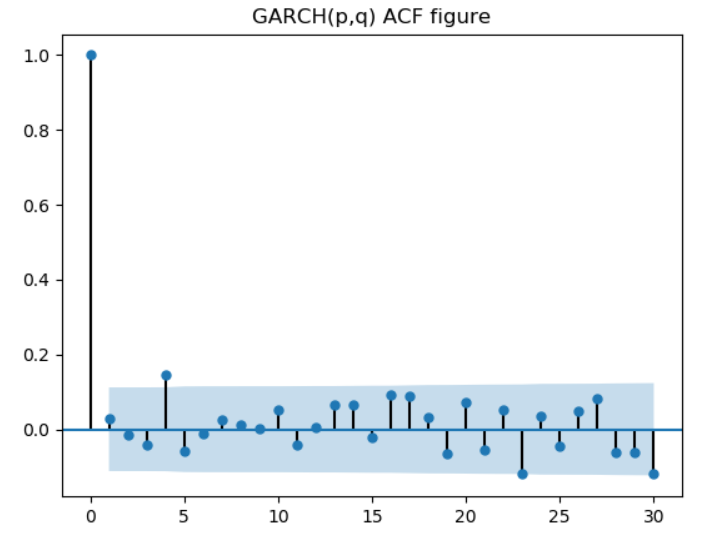
\includegraphics[height=2cm]{images/f000038}
\end{figure}
由图可见,其基本是一个平稳时间序列,可以用来进行预测。但是我们ADF检验表明其是平稳时间序列,但是Ljung-Box检验表明其不是时间平稳时间序列,因此我们还需要仔细分析其中的原因。程序运行结果如下所示:
\begin{figure}[H]
	\caption{程序运行结果}
	\label{f000039}
	\centering
	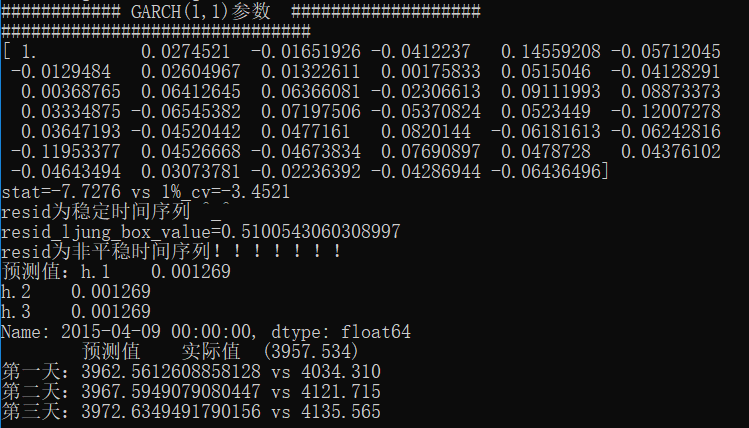
\includegraphics[height=2cm]{images/f000039}
\end{figure}
由上图可以看出,预测结果也基本捕捉到了后三天连涨趋势,只是涨幅估计偏低,这证明我们采用GARCH(p,q)模型来预测是可行的。

